\documentclass[
	9pt, % Set the default font size, options include: 8pt, 9pt, 10pt, 11pt, 12pt, 14pt, 17pt, 20pt
	t, % Uncomment to vertically align all slide content to the top of the slide, rather than the default centered
	%aspectratio=169, % Uncomment to set the aspect ratio to a 16:9 ratio which matches the aspect ratio of 1080p and 4K screens and projectors
]{beamer}

\graphicspath{{Images/}{./}} % Specifies where to look for included images (trailing slash required)

\usepackage{booktabs} % Allows the use of \toprule, \midrule and \bottomrule for better rules in tables
\usepackage{graphicx}
\usepackage{caption}
\usepackage{subcaption}
\usepackage{hyperref}
\usepackage[english,brazil]{babel}
\usepackage{fontawesome5}
\usepackage{listings}
\usepackage{minted}
\usepackage{xcolor}
% \usepackage{graphicx}
% \usepackage{animate}
\RequirePackage[backend=biber,
	style=ieee,
	citestyle=authoryear,
]{biblatex}

% Define a custom command for an icon link
\newcommand{\iconLink}[2]{\href{#1}{\faLink \hspace{0.2em} {#2}}}
\newcommand{\yellowbox}[1]{\colorbox{yellow!75}{#1}}
\definecolor{darkgreen}{rgb}{0,0.5,0}

% Definindo um estilo para o destaque
%----------------------------------------------------------------------------------------
%	SELECT LAYOUT THEME
%----------------------------------------------------------------------------------------
\usetheme{Madrid}

%----------------------------------------------------------------------------------------
%	SELECT COLOR THEME
%----------------------------------------------------------------------------------------

% Beamer comes with a number of color themes that can be applied to any layout theme to change its colors. Uncomment each of these in turn to see how they change the colors of your selected layout theme.

%\usecolortheme{albatross}
%\usecolortheme{beaver}
%\usecolortheme{beetle}
% \usecolortheme{crane}
%\usecolortheme{dolphin}
%\usecolortheme{dove}
%\usecolortheme{fly}
%\usecolortheme{lily}
%\usecolortheme{monarca}
%\usecolortheme{seagull}
%\usecolortheme{seahorse}
%\usecolortheme{spruce}
%\usecolortheme{whale}
%\usecolortheme{wolverine}

%----------------------------------------------------------------------------------------
%	SELECT FONT THEME & FONTS
%----------------------------------------------------------------------------------------
\usefonttheme{default} % Typeset using the default sans serif font

%------------------------------------------------

\usepackage{palatino} % Use the Palatino font for serif text
\usepackage[default]{lato} % Use the Lato font for sans serif text

%----------------------------------------------------------------------------------------
%	SELECT INNER THEME
%----------------------------------------------------------------------------------------
\useinnertheme{rectangles}

%----------------------------------------------------------------------------------------
%	SELECT OUTER THEME
%----------------------------------------------------------------------------------------

% Outer themes change the overall layout of slides, such as: header and footer lines, sidebars and slide titles. Uncomment each theme in turn to see what changes it makes to your presentation.

%\useoutertheme{default}
%\useoutertheme{infolines}
%\useoutertheme{miniframes}
%\useoutertheme{smoothbars}
%\useoutertheme{sidebar}
%\useoutertheme{split}
%\useoutertheme{shadow}
%\useoutertheme{tree}
%\useoutertheme{smoothtree}

%\setbeamertemplate{footline} % Uncomment this line to remove the footer line in all slides
%\setbeamertemplate{footline}[page number] % Uncomment this line to replace the footer line in all slides with a simple slide count

%\setbeamertemplate{navigation symbols}{} % Uncomment this line to remove the navigation symbols from the bottom of all slides

% \bibliography{references} % Specifies the bibliography file to include publications
% \bibliographystyle{apalike} % Specifies the bibliography style
\addbibresource{references.bib}

%----------------------------------------------------------------------------------------
%	PRESENTATION INFORMATION
%----------------------------------------------------------------------------------------

\title[DesWebII]{Desenvolvimento Web II} % The short title in the optional parameter appears at the bottom of every slide, the full title in the main parameter is only on the title page
\subtitle{Aula 09 - Server Sent Events - SSE} % Presentation subtitle, remove this command if a subtitle isn't required
\author[Fabricio Bizotto]{Prof. Fabricio Bizotto} % Presenter name(s), the optional parameter can contain a shortened version to appear on the bottom of every slide, while the main parameter will appear on the title slide
\institute[IFC]{Instituto Federal Catarinense \\ \smallskip \textit{fabricio.bizotto@ifc.edu.br}} % Your institution, the optional parameter can be used for the institution shorthand and will appear on the bottom of every slide after author names, while the required parameter is used on the title slide and can include your email address or additional information on separate lines
\date[\today]{Ciência da Computação \\ \today} % Presentation date or conference/meeting name, the optional parameter can contain a shortened version to appear on the bottom of every slide, while the required parameter value is output to the title slide

%----------------------------------------------------------------------------------------
\begin{document}

%----------------------------------------------------------------------------------------
%	TITLE SLIDE
%----------------------------------------------------------------------------------------

\begin{frame}
	\titlepage % Output the title slide, automatically created using the text entered in the PRESENTATION INFORMATION block above
\end{frame}

%----------------------------------------------------------------------------------------
%	TABLE OF CONTENTS SLIDE
%----------------------------------------------------------------------------------------

\begin{frame}
	\frametitle{Roteiro} % Slide title, remove this command for no title

	\tableofcontents % Output the table of contents (all sections on one slide)
	%\tableofcontents[pausesections] % Output the table of contents (break sections up across separate slides)
\end{frame}

%----------------------------------------------------------------------------------------
%	PRESENTATION BODY SLIDES
%----------------------------------------------------------------------------------------

\section{Server Sent Events - SSE}

\begin{frame}
	\begin{center}

		\bigskip\bigskip\bigskip\bigskip % Vertical whitespace
		{\Large Server Sent Events - SSE}

		\bigskip\bigskip % Vertical whitespace
		{\Huge Uma requisição, uma resposta muito muito longa}

		% \bigskip \bigskip
		% {\small Vamos ver um exemplo prático de CI/CD usando o GitHub Actions}\\
	\end{center}

\end{frame}

\begin{frame}
	\frametitle{Server Sent Events - SSE}
	\framesubtitle{Definição}

	\begin{itemize}
		\item Funcionalidade disponível no protocolo HTTP/1.1 ou superior.
		\item SSE é uma API para criar \textit{streams} de eventos \yellowbox{a partir do
			      servidor} para o cliente.
		\item O cliente recebe notificações do servidor em \yellowbox{tempo real}.
		\item SSE é mais simples de implementar do que \textit{WebSockets}.
		\item Continua sendo uma requisição HTTP, mas a resposta não é fechada.
		\item A diferença para \textit{WebSockets} é que SSE é \yellowbox{unidirecional}.
	\end{itemize}

\end{frame}

\begin{frame}
	\frametitle{Server Sent Events - SSE}
	\framesubtitle{Exemplo de uso}

	\begin{itemize}
		\item O cliente faz uma requisição HTTP para o servidor.
		\item O servidor responde com um cabeçalho \texttt{Content-Type: text/event-stream}.
		\item O servidor envia dados para o cliente \yellowbox{em tempo real}.
		\item O cliente recebe os dados e pode processá-los.
		\item O servidor pode enviar dados para o cliente \yellowbox{a qualquer momento}.
	\end{itemize}

\end{frame}

\begin{frame}
	\frametitle{Server Sent Events - SSE}
	\framesubtitle{Ilustração}

	\begin{figure}
		\centering
		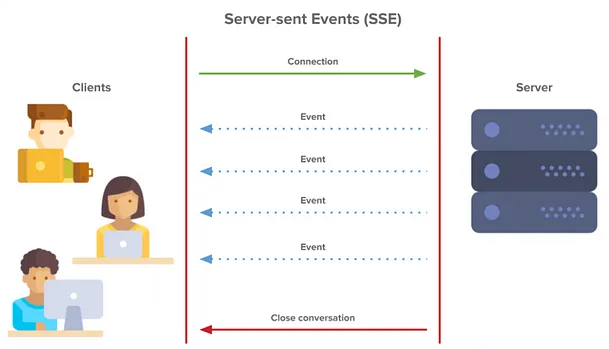
\includegraphics[width=0.9\textwidth]{sse.png}
		\caption{Ilustração de um evento SSE}
	\end{figure}

\end{frame}

\begin{frame}
	\frametitle{Server Sent Events - SSE}
	\framesubtitle{Prós e contras}

	\begin{itemize}
		\item \textbf{Prós}
		      \begin{itemize}
			      \item Simplicidade para real-time.
			      \item \textbf{Padrão W3C}: é compatível com a maioria dos navegadores.
			      \item \textbf{Conexão persistente}: o servidor pode enviar dados sem que o cliente faça uma nova requisição.
		      \end{itemize}
		\item \textbf{Contras}
		      \begin{itemize}
			      \item \alert{Não é bidirecional}. O cliente não pode enviar dados para o servidor.
			      \item Cliente precisa estar \alert{conectado} para receber os eventos.
			      \item \alert{Limite de conexões simultâneas} (6 conexões por domínio), ou seja, o cliente pode abrir no máximo 6 abas para o mesmo domínio.
		      \end{itemize}

	\end{itemize}

\end{frame}

\begin{frame}
	\begin{center}

		\bigskip\bigskip\bigskip\bigskip % Vertical whitespace
		{\Large Server Sent Events - SSE}

		\bigskip\bigskip % Vertical whitespace
		{\Huge Exemplo prático}

		% \bigskip \bigskip
		% {\small Vamos ver um exemplo prático de CI/CD usando o GitHub Actions}\\
	\end{center}

\end{frame}

\begin{frame}
	\frametitle{Server Sent Events - SSE}
	\framesubtitle{Quando usar?}

	\begin{itemize}
		\item \textbf{Notificações em tempo real}: por exemplo, notificações de novas mensagens em um chat.
		\item \textbf{Atualizações em tempo real}: por exemplo, atualizações de preços de ações.
		\item \textbf{Atualizações de dados}: por exemplo, atualizações de dados de sensores.
		\item \textbf{Atualizações de progresso}: por exemplo, progresso de um upload de arquivo.
		\item \textbf{Atualizações de eventos}: por exemplo, atualizações de eventos em um jogo.
	\end{itemize}

\end{frame}

\begin{frame}
	\frametitle{Server Sent Events - SSE}
	\framesubtitle{Exemplo prático}

	\begin{figure}
		\centering
		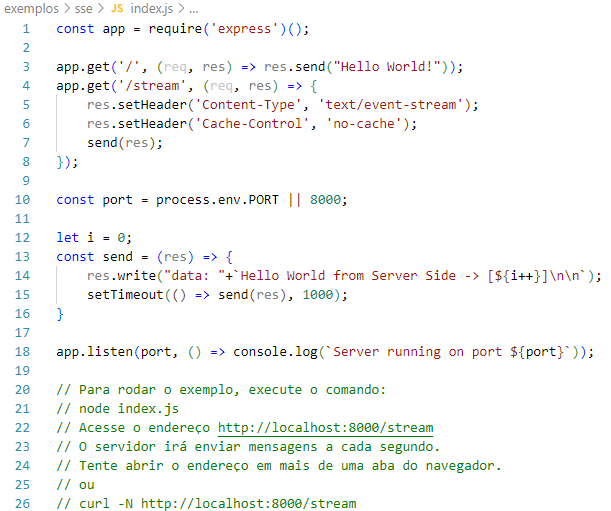
\includegraphics[width=0.7\textwidth]{sse_example.png}
		\caption{Exemplo prático de uso de SSE}
	\end{figure}

\end{frame}

\begin{frame}
	\frametitle{Server Sent Events - SSE}
	\framesubtitle{Exemplo prático}

	\begin{itemize}
		\item Vamos ver um exemplo prático de uso de SSE.
		\item O exemplo será feito em Node.js para simular uma lista de chamadas dos alunos.
		\item O exemplo será disponibilizado em
		      \textbf{\href{https://github.com/fabricioifc/sse-votes}{https://github.com/fabricioifc/sse-votes}.}
	\end{itemize}

\end{frame}

\section{Experimentos}

\begin{frame}
	\frametitle{Server Sent Events - SSE}
	\framesubtitle{Experimentos}

	Escolha um dos exercícios a seguir para implementar um exemplo prático de uso
	de SSE: \bigskip

	\begin{enumerate}
		\item \textbf{Exercício 1}: Contador de votos em tempo real.
		\item \textbf{Exercício 2}: Chat em tempo real.
		\item \textbf{Exercício 3}: Sistema de notificações em tempo real.
		\item \textbf{Exercício 4}: Sistema de atualização de dados em tempo real.
		\item \textbf{Exercício 5}: Contador de visitas em tempo real.
		\item \textbf{Exercício 6}: Sistema leilão em tempo real.
		\item \textbf{Exercício 7}: Sistema de lista de compras colaborativa em tempo real.
		\item \textbf{Exercício 8}: Sistema de rastreamento de entregas em tempo real.
		\item \textbf{Exercício 9}: Outros sistemas em tempo real.
	\end{enumerate}

\end{frame}

\end{document}
